\section{Características del conjunto de datos} \label{specs}

	Además de los filtros aplicados mencionados en la sección \ref{filtro}, se aplican filtros adicionales sobre la energía y el rango de tiempo. Para estudiar los eventos en esta sección, consideramos los eventos entre 1\,EeV y 2\,EeV de energía y que ocurrieron entre las 12:00:00 GMT del 1 de enero de 2014 y las 12:00:00 GMT del 1 de enero de 2020. Se centró en este rango de tiempo porque entre hasta fines del año 2013, la tasa de eventos estuvo por debajo de la media de los años siguientes como se muestra en la Fig.\,\ref{fig:rate_2020_AllTriggers}. Además que el registro de eventos más reciente al que se tuvo para hacer este trabajo termina el 1 de Enero del 2020  a las 11:59:43 GMT, además de para estudiar una cantidad entera de años, se optó por considerar los eventos desde el 1 de Enero del 2014 a las 12:00:00 GMT.

    \begin{figure}[H]
    	\centering
    	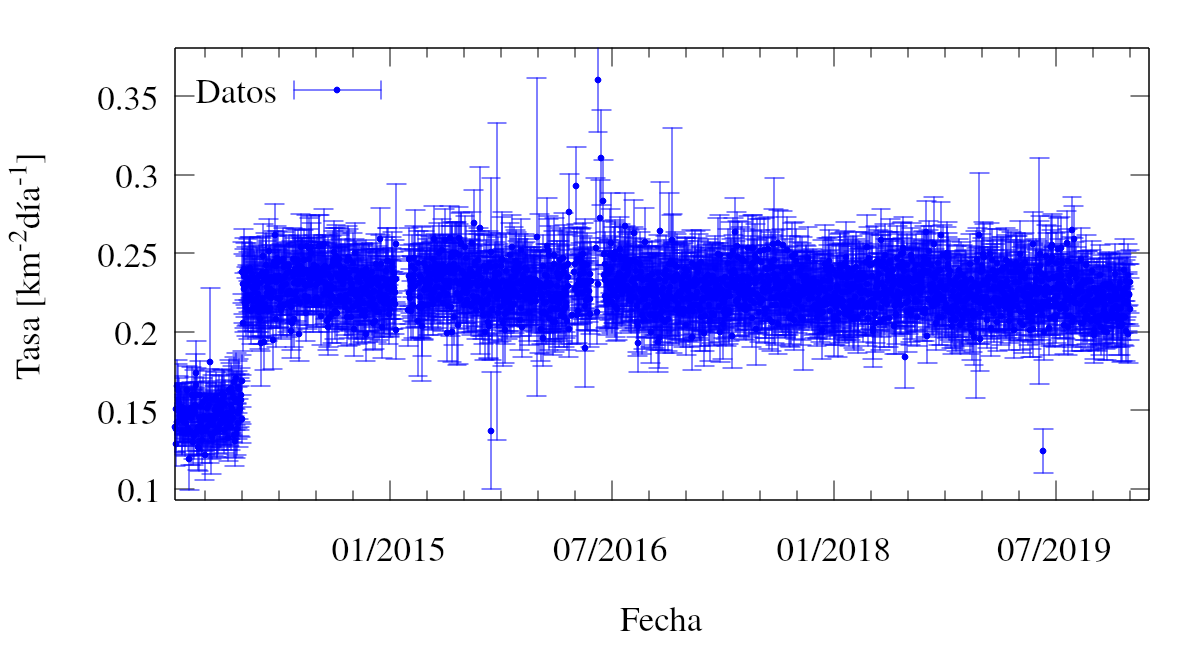
\includegraphics[width=0.75\textwidth]{rate_over_1-2_EeV-theta-60.png}
    	\caption{Tasa de eventos del conjunto más reciente de eventos con todos los disparos. Se observa un tasa baja en la segunda mitad del 2013.}
    	\label{fig:rate_2020_AllTriggers}
    \end{figure}

	Un resumen de todos los filtros aplicados se encuentra a continuación
		\begin{enumerate}
			\item Son eventos obtenidos mediante todos los disparos.
			\item Energía entre  [1 EeV , 2 EeV)
			\item Rango de tiempo:
			\begin{itemize}
				\item[-] Inicial:Jueves, 1 de Enero de 2014 12:00:00 GMT o 1388577600 UTC
				\item[-] Final:  Jueves, 1 de Enero de 2020 12:00:00 GMT o 1577880000 UTC
			\end{itemize}

		\end{enumerate}
	Aplicando estos filtros, se tienen $1\,081\,844$ eventos para estudiar en este rango de energía. 

    Se debe tener cuenta que el archivo de evento para todos los disparos tiene diferencias con el conjunto de eventos del disparo estándar. Porque el primero es entre los años 2013 y 2019 y el segundo se adquieren usando el disparo estándar entre los años 2004 y 2018.  Algo a considerar es que la colaboración cambió el algoritmo de reconstrucción de eventos en el 2019, con respecto a la versión del 2017.  

    En las  Figs.\,\ref{fig:deltaE} y \ref{fig:histograma} se muestra la diferencia entre las energías de la reconstrucción del año 2017 $E_{2017}$ de archivo de todos los disparos, que sigue sin ser corregida por los parámetros del clima, y la energía de último conjunto de datos $E_{2019}$, que ya fue corregida la modulación del clima y reconstruida por el nuevo algoritmo. Las variables utilizadas en las figuras son $\Delta E = E_{2019} - E_{2017}$ normalizada por la energía media $\langle E \rangle= (E_{2019} +  E_{2017})/2 $ para energías entre 1 EeV y 2 EeV de los dos conjuntos de datos. Se consideran eventos coincidentes entre las reconstrucciones del año 2017 y 2019. Puede apreciarse que la diferencia no esta centrada 0 y aparenta tener una modulación del clima. La amplitud de esta modulación es pequeña respecto al valor medio de $\Delta E$. Por lo tanto la diferencia entre ambos conjuntos se debe a una reconstrucción distinta de los eventos. 

        \begin{figure}[H]
          \centering
            \begin{subfigure}[b]{0.5\textwidth}
              \centering
              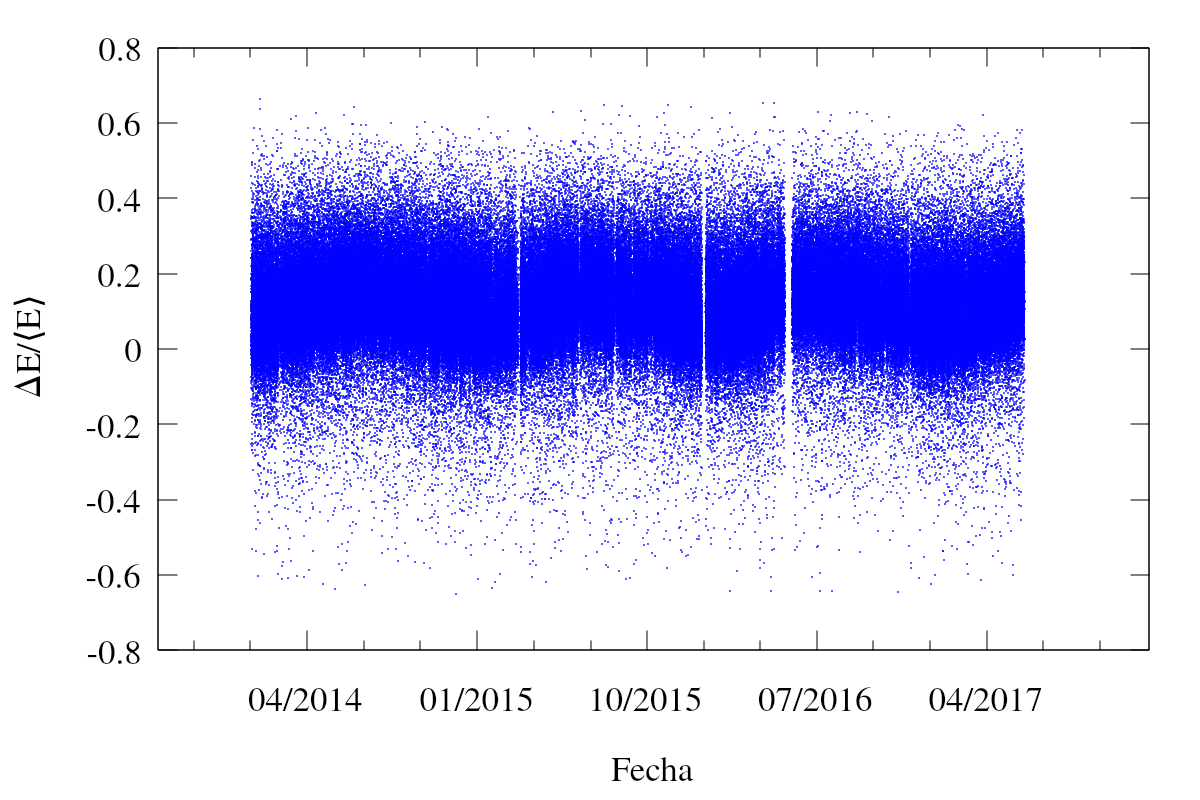
\includegraphics[width=\linewidth]{deltaE_tiempo_v2_rango_1_2.png}
              \caption{Diferencia entre las energías} \label{fig:deltaE}
            \end{subfigure}%
            \begin{subfigure}[b]{0.5\textwidth}
              \centering
              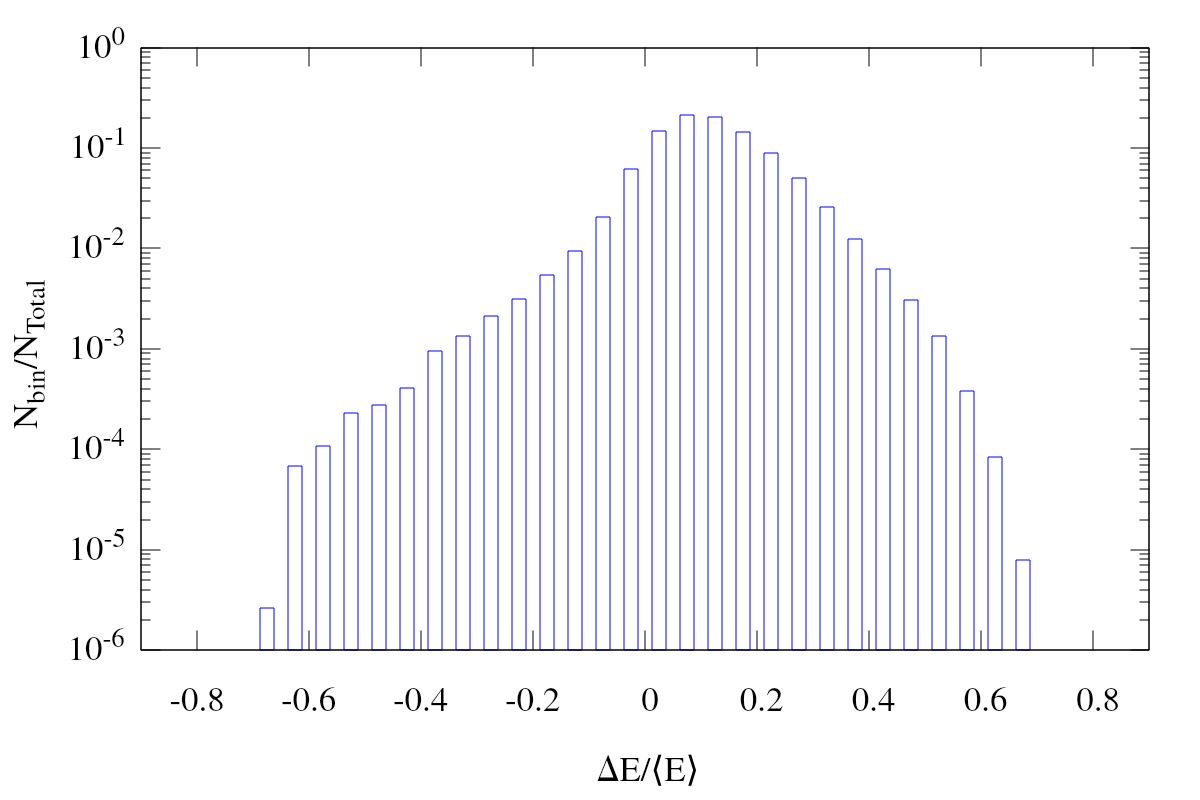
\includegraphics[width=\linewidth]{histograma_deltaE_v3_rango_1_2.png}
              \caption{Histograma de las diferencias}   \label{fig:histograma}
            \end{subfigure}
           \caption{Diferencia entre las energías de entre la reconstrucción del 2017 y del 2019}
         \end{figure}
	
\subsection{Pesos de los eventos para frecuencias de referencia}

En la Fig.\,\ref{pesos_bin_1_2} se muestran los valores de  $\Delta N_{cell,k}(\alpha^0)$ en función de la ascensión recta del cenit del observatorio, en el rango mencionado en la sección anterior \ref{specs}, para frecuencias de referencia. 
			 
			\begin{figure}[H]
				\centering
				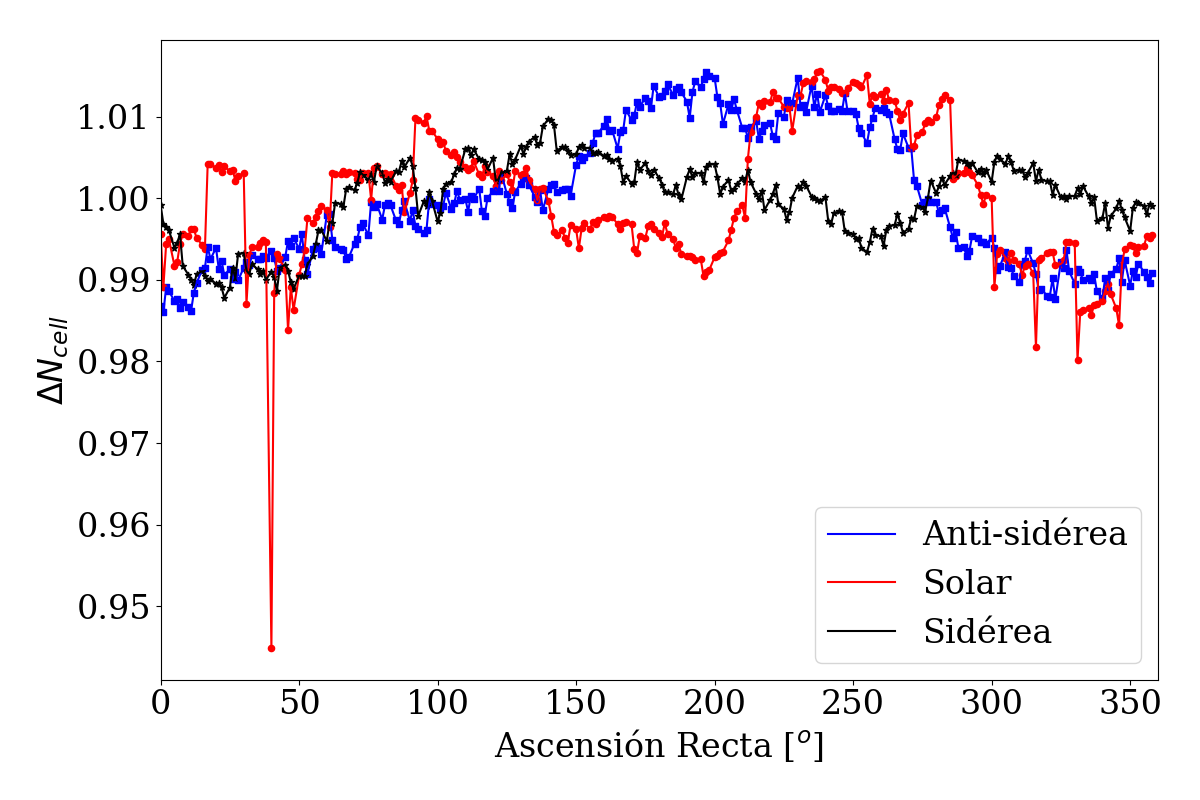
\includegraphics[width=0.6\textwidth]{weights_2013_2020.png}
				\caption{Variaciones de los hexágonos en función de la ascensión recta del observatorio para frecuencias características en rango mencionado. }
				\label{pesos_bin_1_2}
			\end{figure}


\section{Análisis de anisotropías en ascensión recta para el primer armónico}

En la Fig.\ref{anisotropia_rayleigh} se muestra en barrido de frecuencias para la amplitud del primer armónico de Fourier. Se marcan con líneas verticales las frecuencias de referencia mencionadas anteriormente. Se observa el barrido sin considerar las correcciones por las variaciones de los hexágonos con una línea discontinua. La  amplitud  en la frecuencia solar sin la corrección de los pesos es importante. Un ejemplo de errores sistemáticos puede ser que en épocas invernales el acceso a los tanques se dificulta y ponerlos en funcionamento nuevamente tras una tormenta o para un cambio de baterías puede llevar más tiempo que durante verano. 

		\begin{figure}[H]
			\centering
			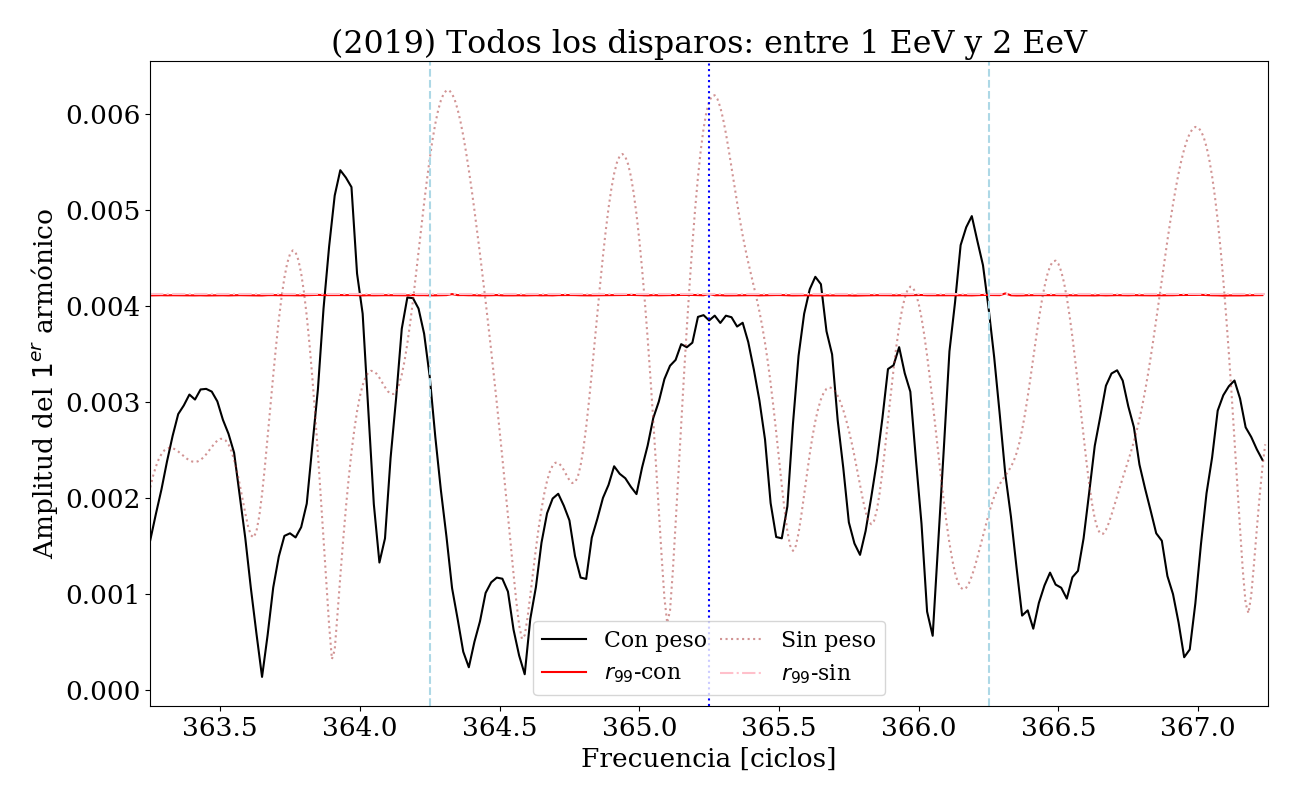
\includegraphics[width=0.85\linewidth]{pesos_sin_con_1_2_EeV.png}
			\caption{Anisotropía en función de la frecuencia para el rango de energía 1  EeV - 2 EeV. Se comparan los análisis sin los pesos y con los pesos de los hexágonos entre en 1 de Enero del 2014 y el 1 de Enero del 2020}
			\label{anisotropia_rayleigh}
		\end{figure}

Cuando se consideran los pesos, está amplitud disminuye y pasa a estar por debajo del umbral de $\tilde{r}_{99}$, y aparecen dos amplitudes por encima de este umbral: un pico es la frecuencia sidérea, donde buscamos las anisotropías en ascensión recta, y otro pico es cerca de la frecuencia anti-sidérea, que indica que existen componentes de errores sistemáticos sobre los datos que deben ser considerados. Por ejemplo, la corrección de clima que se analiza en el trabajo de licenciatura se realiza sobre el disparo estándar, se podría calcular los parámetros del clima utilizando los eventos de todos los disparos y comprobar si esto disminuye la amplitud del primer armónico de la frecuencia cercana a la anti-sidérea.

		
En la Tabla\,\ref{table:parametros_rayleigh} se resumen las amplitudes y fases obtenidas mediante el análisis a primer orden en Fourier. Se
		\begin{table}[H]
		\centering
		\begin{tabular}{|l|l|l|l|l|}
			\cline{2-5}
			\multicolumn{1}{c|}{} & \multicolumn{2}{c|}{Sin pesos} 		& \multicolumn{2}{c|}{Con pesos} \\ \hline
			Frecuencia:           & Solar          & Sidérea       		& Solar         & Sidérea        \\ \hline
			Fase $\phi$:          & $(251\pm13)^o$ & $(289\pm40)^o$		& $(288\pm20)^o$& $(337\pm19)^o$            \\ \hline
			Amplitud $r$:         & 0.0061         & $0.0018\pm0.0001$  & $0.0039\pm0.0001$      & $0.0040\pm0.0001$         \\ \hline
			$P(r)$:               & 0.0038 \%      & 41\%          		& 1.8 \%        & 1.3 \%       \\ \hline    
		\end{tabular}
		\caption{Comparación de los parámetros de fase y amplitud para las frecuencias sidérea y solar, analizando sin pesos y con los pesos de los hexágonos con el análisis de Rayleigh entre en 1 de Enero del 2014 y el 1 de Enero del 2020}
		\label{table:parametros_rayleigh}
		\end{table}


Las Fig.\,\ref{fig:bin_events_first_order} se muestra la tasa de eventos normalizada con pesos y sin pesos para este rango de energía. Las líneas discontinuas representan los parámetros de la Tabla\,\ref{table:parametros_rayleigh} para el primer armónico del análisis de Rayleigh de la frecuencia sidérea. Se observa que la modulación de los eventos con y sin pesos tiene características que la aproximación a primer orden no refleja. 	En las Fig.\,\ref{fig:bin_events_second_order_con} se muestra la tasa de eventos con pesos y el ajuste hasta el segundo orden en Fourier, en el mismo se muestra que este orden refleja mejor las características de los datos. Los resultados del análisis de Rayleigh  se muestran en la Tabla\,\ref{table:parametros_second_order}
	\begin{figure}[H]
		\centering
		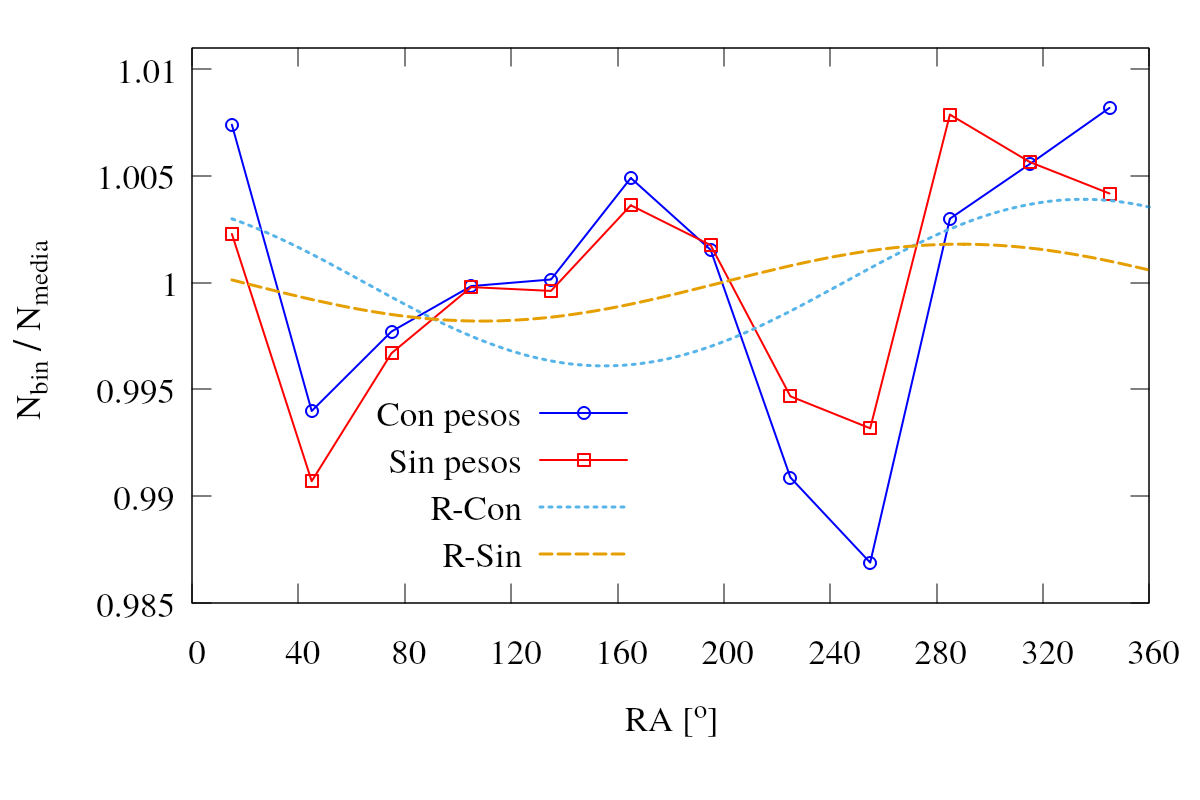
\includegraphics[width=0.65\linewidth]{eventos_clasificados_por_RA_v4.png}
		\caption{Distribución de la cantidad relativa de eventos en función de la ascensión recta a primer orden, en el rango de energía $1$ EeV - $2$ EeV.}
		\label{fig:bin_events_first_order}
	\end{figure}

        \begin{figure}[H]
          \centering
            \begin{subfigure}[b]{0.5\textwidth}
		\centering
		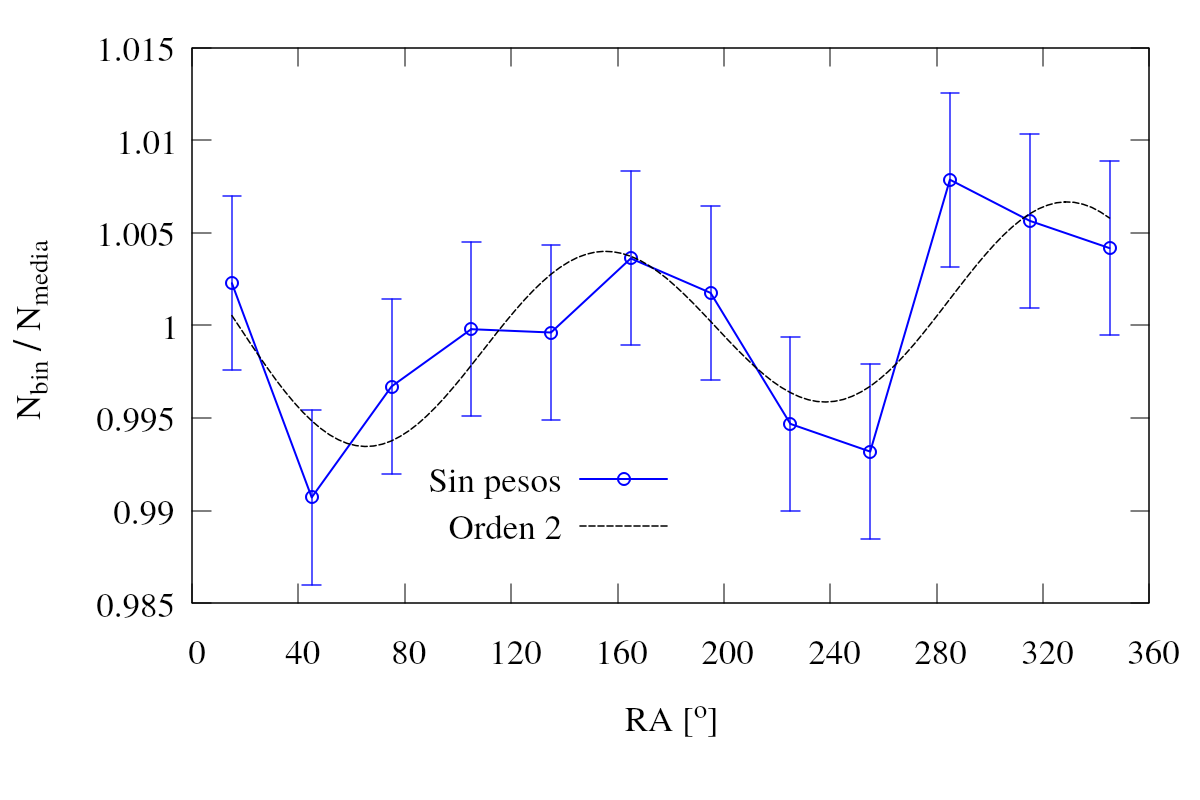
\includegraphics[width=\linewidth]{eventos_clasificados_por_RA_v7_orden_2_sin_pesos.png}
		\caption{Eventos sin pesos}		\label{fig:bin_events_second_order_sin}
            \end{subfigure}%
            \begin{subfigure}[b]{0.5\textwidth}
		\centering
		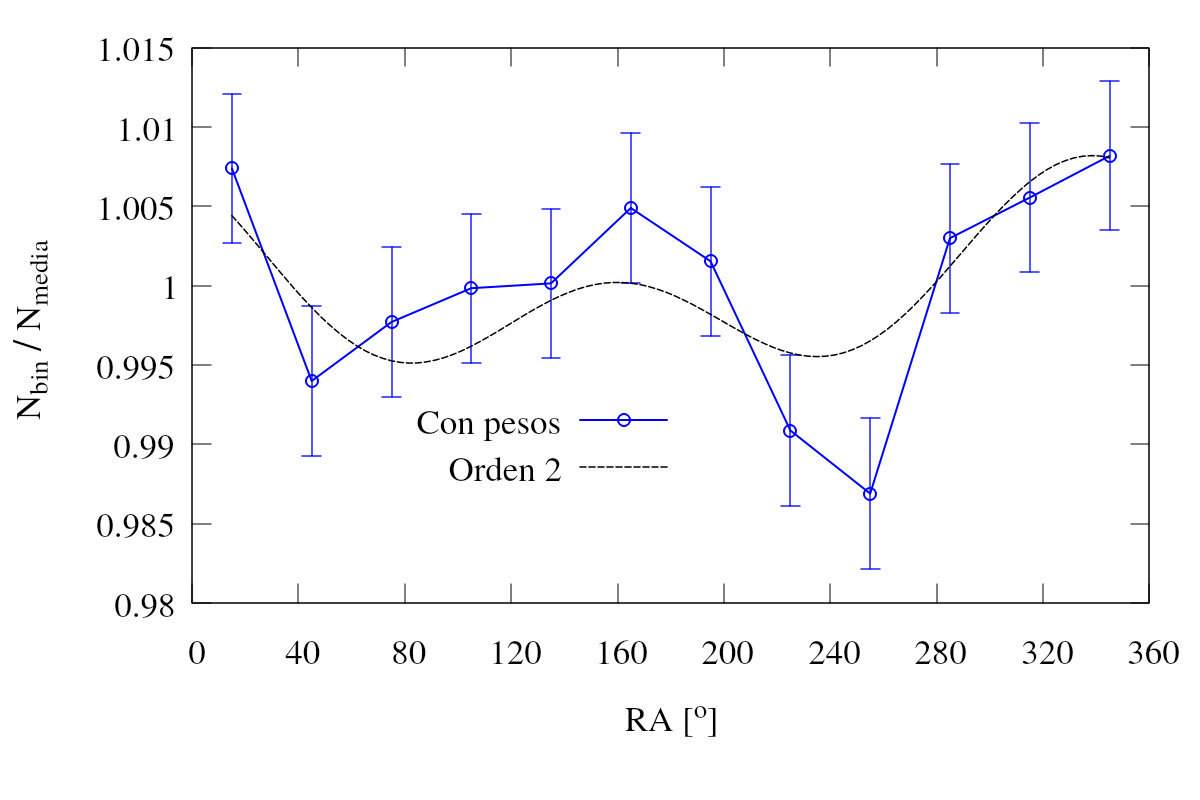
\includegraphics[width=\linewidth]{eventos_clasificados_por_RA_v7_orden_2_con_pesos.png}
		\caption{ Eventos con sus respectivos pesos}		\label{fig:bin_events_second_order_con}
            \end{subfigure}
           \caption{Distribución de la cantidad relativa de eventos en función de la ascensión recta a segundo orden en el rango de energía $1$ EeV - $2$ EeV entre en 1 de Enero del 2014 y el 1 de Enero del 2020.}
         \end{figure}

		\begin{table}[H]
		\centering
			\begin{tabular}{l|l|l|}
			\cline{2-3}
			                                      & Sin Pesos 		 & Con Pesos \\ \hline
			\multicolumn{1}{|l|}{Orden k :}       & 2                & 2                    \\ \hline
			\multicolumn{1}{|l|}{Fase $\phi_k$:}  & $(153\pm8)^o$    & $(170\pm9)^o$                   \\ \hline
			\multicolumn{1}{|l|}{Amplitud $r_k$:} & $0.0054\pm0.0001$& $0.0041\pm0.0001$               \\ \hline
			\multicolumn{1}{|l|}{$P(r_k)$:}       & $0.039$\%        & 1.0\%  \\ \hline
			\end{tabular}
		\caption{Parámetros obtenidos del ajuste a segundo orden con el análisis de Rayleigh.}
		\label{table:parametros_second_order}
		\end{table}

\subsection{Trabajo a futuro}

%Los resultados obtenidos en este rango de energía sugieren la existencia de un dipolo en ascensión recta, ligeramente corrido del centro galáctico que se encuentra alrededor de $260^o$, que proveería información sobre la transición galáctica - extra galáctica de las fuentes de los RCs de ultra alta energía.

La modulación del primer armónico de los eventos entre 1 EeV y 2 EeV tiene amplitudes por encima del umbral de $r_{99}$ para varias frecuencias, por lo que no puede decirse nada concreto sobre la existencia del dipolo en ascensión recta.


Durante el próximo semestre se trabajará en tratar de mejorar la calidad de los datos, en primer lugar implementando una corrección de los efectos climáticos a partir del conjunto de datos con todos los disparos.
%Para confirmar o desmentir  esto, durante el siguiente semestre trabajará en corregir la modulación del clima sobre los eventos, y verificar si el pico cercana a la frecuencia anti-sidérea que está por encima del umbral de $r_{99}$ puede disminuir.